\documentclass[twocolumn]{article}

\usepackage{tabularx}

\usepackage{titlesec}

% Center section titles
\titleformat{\section}{\centering\large\bfseries}{\thesection}{1em}{}

\renewcommand{\thesection}{\Roman{section}} % set section numbering to Roman numerals

\usepackage{multicol}

\usepackage{graphicx}
\graphicspath{{images/}}

\usepackage[margin=2cm]{geometry}

%HyperLinks for Table of Contents
\usepackage{hyperref}
\hypersetup{colorlinks = true, citecolor = blue, linkcolor = blue, urlcolor = blue}

%Starting of the Document
\begin{document}
%Title will go over here
\begin{titlepage}
\newgeometry{margin=3cm} % Change margins for the title page only
    \centering
     \onecolumn
    {\huge\bfseries A Smart Way to Detect Health Conditions from Blood Report using\\ Machine Learning\par}
    \vspace{0.5cm}
    \Large \textbf{$^1$N. Ramesh Babu\\}rameshbabun@rguktsklm.ac.in\\
  \begin{multicols}{2}
   \Large \textbf{$^2$K. Manoj Kumar\\}s170936@rguktsklm.ac.in\\
    \Large \textbf{$^3$B. Prem Kumar\\}s170456@rguktsklm.ac.in\\
     \Large \textbf{$^4$N. Kishorekumar\\}s170095@rguktsklm.ac.in\\
      \Large \textbf{$^5$K. Umamaheswari\\}s170314@rguktsklm.ac.in\\
  
  \end{multicols}
    \vspace{0.5cm}
    {\large Date: \today \par}
    \vspace{0.2cm}
    \begin{figure}[h]
	\centering
	
\includegraphics[scale=0.7]{rgukt_logo.jpg}
	\end{figure}
	\vspace{0.2cm}
   
    \vspace{0.5cm}
    {\Large\itshape Department of \textbf{Electronics and Communication Engineering}\par}
    \vspace{0.5cm}
   {\Large\textsc{Rajiv Gandhi university of Knowledge Technologies, Srikakulam}\par}
    \vspace{2cm}
    \begin{flushright}
    {\large Date: \today \par}
    \end{flushright}
\end{titlepage}

\pagebreak
\onecolumn
\tableofcontents %for making table of contents
\clearpage

\twocolumn
%Abstract
\begin{center}
\section*{Abstract}
\end{center}
\addcontentsline{toc}{section}{ABSTRACT}
This project aim is to detect complications in the blood. Nowadays blood analysis plays a major role in the pharmaceutical world. Blood analysis is very essential to treat any disease. Blood report consists of various measures like red and white blood cells, platelets count and hemoglobin etc. The blood analysis report is one of the main reports in the medical field to analyse the health of a patient. Doctors use this report to understand the health condition of a patient to give medication and to perform any surgery. In the Blood measure report, every measure has some range to maintain our body healthy. By this range, we can get an idea about which measure is not in range or deficit in range. So, it is a very crucial thing to understand the condition accurately and effectively. Nowadays, most people are becoming sick and hospitals are becoming crowded. At that time the hospital staff or doctors can upload the report to get a perfect analysis. The project aims to extract the information from the uploaded report using OCR and to apply an ML algorithm to that extracted values to detect complications in the blood and gives the result through the designed website. \cite{Allison1996}\\

\begin{flushleft}
\textbf{{\large Keywords:}\\}
\end{flushleft}
 Blood report, Optical Character Recognition (OCR), ML algorithm, Web-Framework, file operations\\

\section{INTRODUCTION}
Blood is one of the major components of the human body. Like organs, blood is very important. Blood contains different types of parameters like Haemoglobin, Red blood cells, White blood cells, Platelets etc.., Each parameter has its range of values. The changes in these values can affect the  human and may cause diseases. Changes in different parameters can cause different types of diseases. There are various types of diseases, which can be caused by changes in the blood. The range of values will vary based on age and gender also.

Analysing the blood report is the major step to detect the health condition of a patient. Most of the blood tests don’t need special conditions like fasting etc., Blood tests can be done at any time. Different parameters can be measured by testing blood. The results will help to identify health problems in the early stages. Only a blood test is not enough to deal with a patient’s health condition, but it’s one of the factors. Applying modern technology to our daily life work will reduce human effort and can increase accuracy. Applying modern technologies like Machine Learning and Artificial Intelligence is a hot topic nowadays

Machine Learning is a data analysis technology that teaches computers to act like humans. It’s a data-driven technology, it works based on the dataset given to it. The performance of the machine learning algorithm can be improved according to the dataset provided. The main objective of this project is to predict the health condition of a patient from their blood report. Different Machine Learning algorithms are used to get an algorithm with maximum accuracy. 

Getting results through an interface is also important for the project. Creating 2 webpages, in which, one is to upload our document or photo of the report and another is to show the results.

The rest of the paper is organized as follows. Section II introduces background information about the used techniques. Section III presents the different related methods of blood disease prediction using ML classifiers. Section IV describes the data set and the blood test attributes. Section V shows the results of the experiment. Section VI presents the website, which we are going to display results through. Finally, section VII presents the conclusion and future work of the research.

\section{BACKGROUND} 
Machine learning is a computer science branch that is responsible for the development of computer systems that can learn and change their actions according to the situation. Machine Learning technology is depending on learning from the data-set given to it and evaluating the model results and trying to optimize the output. Fig.\ref{mlactivity} Shows a brief detailing of the machine learning activity. There are three types of algorithms. They are: 

\begin{itemize}
\item Supervised Learning: The computer trained with presented inputs and  their desired outputs, for predicting the output of future inputs. 
\item Unsupervised Learning: The computer presented with inputs without desired outputs. 
\item Reinforcement learning: The computer interacts with the environment, and it must perform a specific goal without training. 
\end{itemize}

\begin{figure}[ht]
\centering
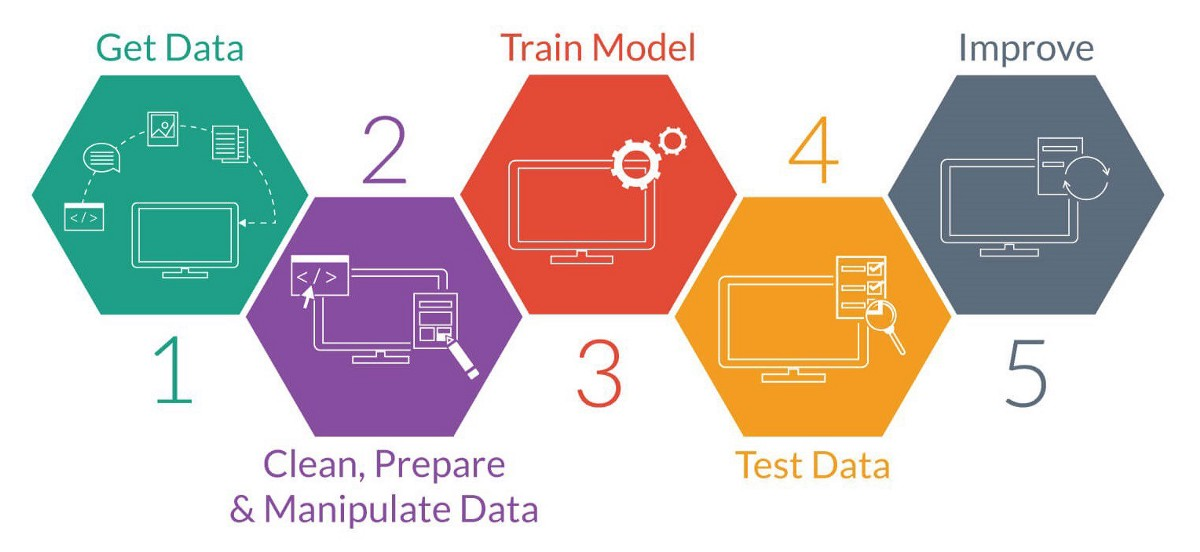
\includegraphics[scale=0.25]{figure1.png}
\label{mlactivity}
\caption{Machine Learning Activity}
\end{figure}


Machine Learning techniques become an essential tool for prediction and decision-making in many disciplines. The availability of clinical data leads machine learning to play a critical role in medical decision-making. It serves as a valuable aid in identifying a disease for improving clinical decisions and choosing suitable medical procedures.

\begin{center}
\section{CLASSIFIERS USED}
\end{center}

We used the following classifiers for classifying the patients based on learning datasets; these classifiers are:
\begin{itemize}

\item Random forests classifier: it is a band learning method for classification that operates by constructing a multitude of decision trees by training records with their labelled classes. After building the tree, the unknown records could be classified.
\addcontentsline{toc}{subsection}{Random forests classifier}

\item Support vector machine: it represents the training data as points in a flat separated space by an apparent gap. New examples are mapped into space with the forecast category based on which side of the gap they fall. 
\addcontentsline{toc}{subsection}{Support vector machine}

\item Decision Tree: it models the attributes and their values with decisions in the tree; where the nodes contain attributes with their values and leaves contain decisions. The algorithm considers all features and makes a binary split on them. It orders the attributes on the tree according to the information gain value in descending order. After building the tree, new tuples will be classified according to their values by traversing the tree until reaching the leaf that contains the class.
\addcontentsline{toc}{subsection}{Decision Tree}
\end{itemize}
All these classifiers are used in the disease prediction process for improving clinical decision-making and minimizing medical errors, in the next section, we listed the recent research that uses machine learning in blood disease analysis.

\section{DATA SET and DISEASES}
The dataset on which the ml model is trained is created after a lot of research. Creating a dataset is the major part of this project. The dataset contains 4,500 data points and 15 classes. Each class contains 300 data points. Each class has values based on the age and gender of the patient. Each class represents each disease.
These are the diseases that ml model is going to predict.\cite{Safavian1991}
\begin{itemize}


\item\textbf{Anaemia:} it is a decrease in the amount of haemoglobin or red blood cells in the blood. It may cause vague and may include feeling tired, shortness of breath, or weakness.\cite{Cabitza2017}
Based on the count, it has four types:

\begin{enumerate}
\item Mild Anaemia
\item Moderate Anaemia
\item Severe Anaemia
\item Dangerous Anaemia
\end{enumerate}

\item\textbf{Polycythaemia:} an abnormally high amount of haemoglobin or red blood cells in the blood. 
\item\textbf{Thrombocytopenia:}it is about the lack of platelets. It is not so dangerous but sometimes leads to bleeding too much.
Based on the count, it has four types:

\begin{enumerate}
\item Mild Anaemia
\item Moderate Anaemia
\item Severe Anaemia
\item Danger
\end{enumerate}

\item\textbf{Thrombocytosis:} an abnormally high number of Platelets in blood.

\item\textbf{Leucocytosis:} it causes an increase in white cells above the normal range in the blood. It may cause certain parasitic infections or a tumour, as well as leukaemia. 

\item\textbf{Leukopenia:} it causes a decrease in white cells below the normal range in the blood. 

\item\textbf{Neutrophilia:} is defined as a higher neutrophil count in neutrophil count in the blood than normal. Neutrophilia can bee is seen in infections and inflammation.

\item\textbf{Neutrophilia:} It can be caused by diseases that damage the bone marrow, infections or certain medications.

\item\textbf{Eosinophilia:} High eosinophilia levels can indicate a mild condition such as a drug reaction or allergy.

\item\textbf{Basophilia:} Basophilia may be a sign you have an infection, or it may be a sign of serious medical conditions like leukaemia. 

\item\textbf{Monocytosis:} Having an abnormally high number of infection-fighting monocytes. It may signify a severe medical condition such as an autoimmune disease, a blood disorder, or cancer. It may also mean that you have encountered an infection.\cite{Darcy2016}

\item\textbf{Lymphocytosis:} Causes when we have high lymphocytes count. Lymphocytosis is one of the first signs of certain blood cancers.

\item\textbf{Normal:} in this class, all parameters’ values are normal, and there are no essential notifications in the blood analysis.\cite{Jiang2011}

\end{itemize}

\begin{table*}[ht]
\centering
\begin{tabularx}{\textwidth}{|X|X|}
\hline
\textbf{Parameters} & \textbf{Description} \\
\hline
Age &Age of the patient \\
\hline
Gender& Gender of the patient \\
\hline
HGB&Haemoglobin\\
\hline
Thrombocytes& Platelets Count (in Millions) \\
\hline
Leukocytes& White Blood cells count \\
\hline
Neutrophil & Per cent Neutrophils in blood \\
\hline
Eosinophil & Per cent of Eosinophils in blood\\
\hline
Basophil &Per cent of Basophils in blood\\
\hline
Lymphocyte &Per cent of Lymphocytes in blood\\
\hline
Monocyte &Per cent of Monocytes in blood\\
\hline
\end{tabularx}
\caption{BLOOD ANALYSIS PARAMETERS}
\label{tab:example}
\end{table*}


\section{EXPERIMENT RESULTS AND DISCUSSION}

Cross-validation is a statistical method of evaluating and comparing learning classifiers by dividing data into parts: one is training data, which is used to train the model. Second is testing data, the model is used to validate the model. The training and testing sets must cross over in successive rounds such that each data point has a chance of being validated.\cite{Michalski1990}

For each classifier, accuracy is measured. The Random Forest algorithm provides high accuracy and SVM provides less accuracy than Random Forest. The overall results prove the success of applying classical machine learning algorithms in the process of blood disease prediction.

\begin{table}[ht]
\centering
\begin{tabular}{|c|c|}
\hline
\textbf{Classifier} & \textbf{Accuracy} \\
\hline
SVM & 98\% \\
\hline
Decision Tree & 99\% \\
\hline
Random Forest & 100\% \\
\hline
\end{tabular}
\caption{Accuracy Results for each classifier}
\label{tab:example2}
\end{table}

\begin{figure}[ht]
\centering
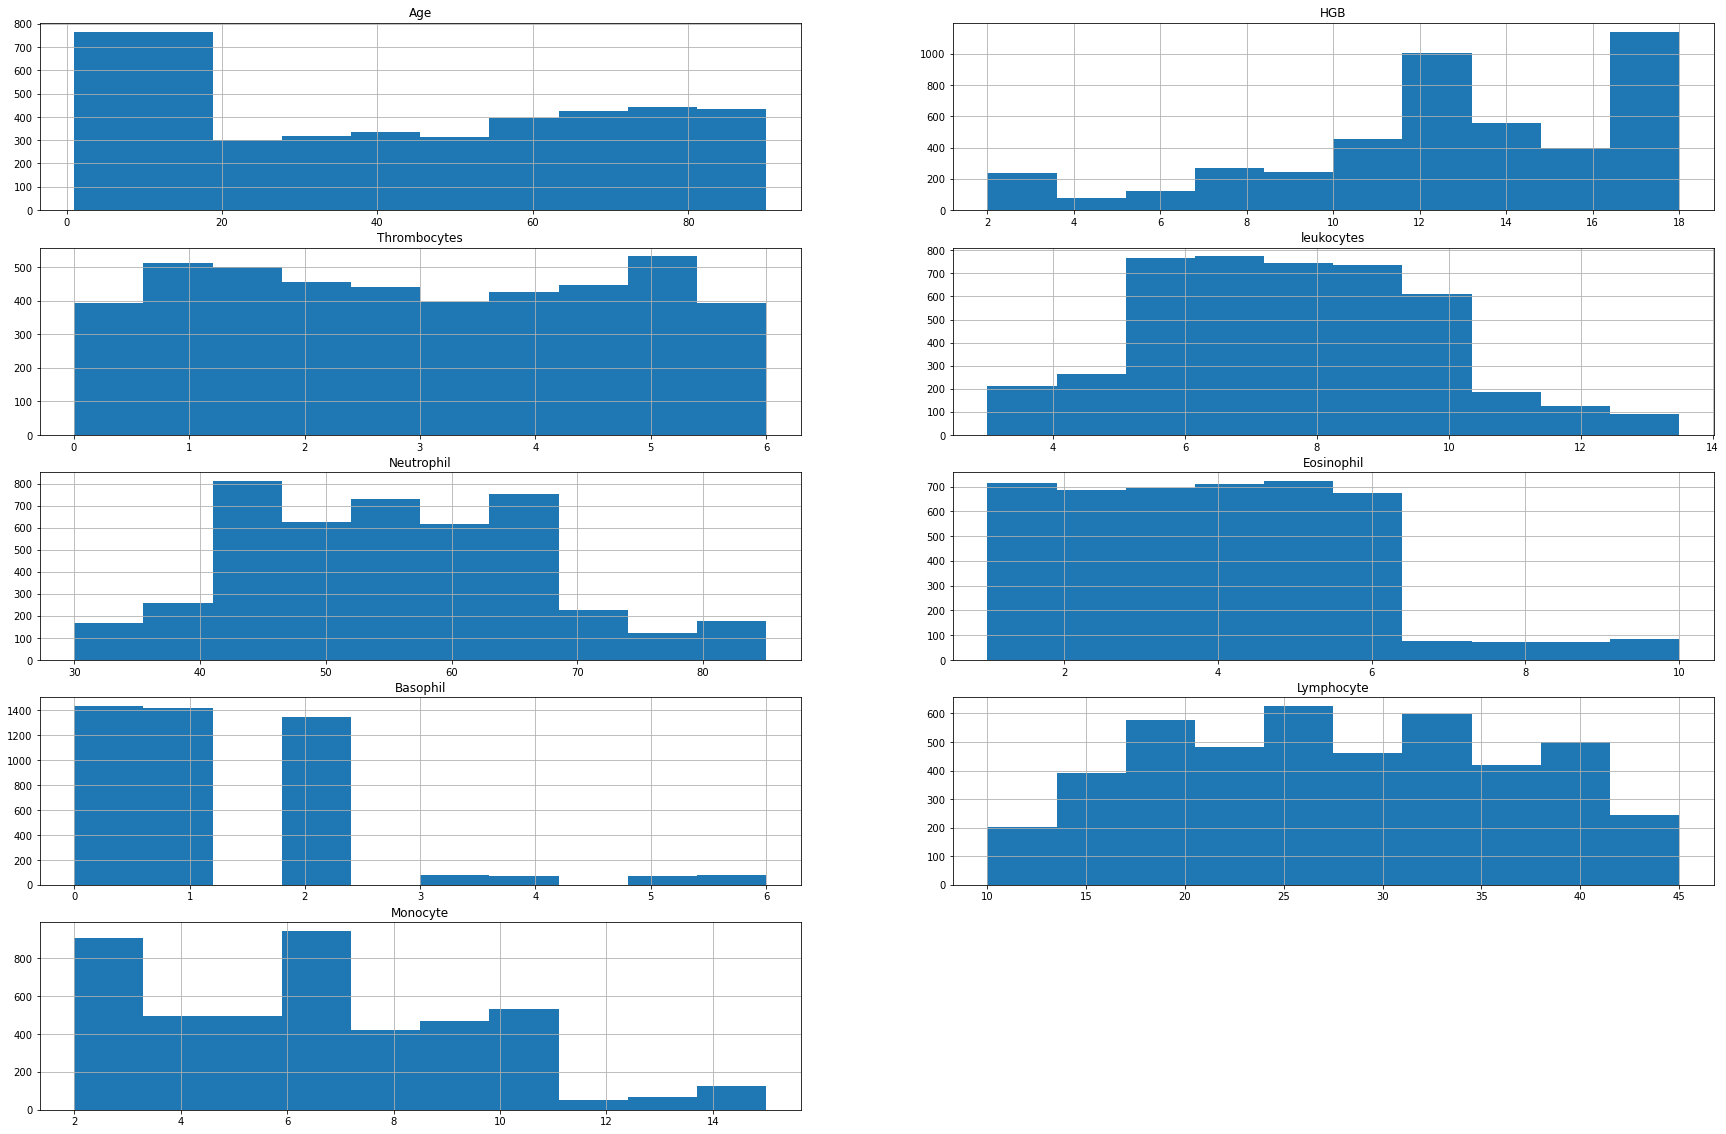
\includegraphics[scale=0.15]{figure2.png}
\label{histogram}
\caption{Histogram for each feature}
\end{figure}
\vspace{2cm}
\begin{figure}[ht]
\centering
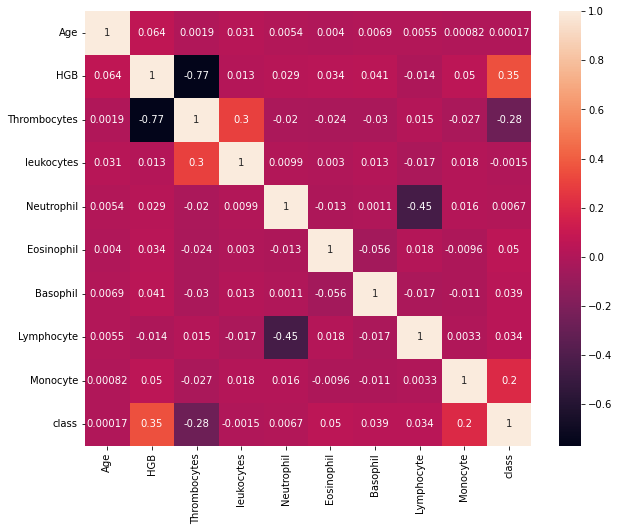
\includegraphics[scale=0.37]{figure3.png}
\label{heatmap}
\caption{Heat Map}
\end{figure}

\begin{figure}[ht]
\centering
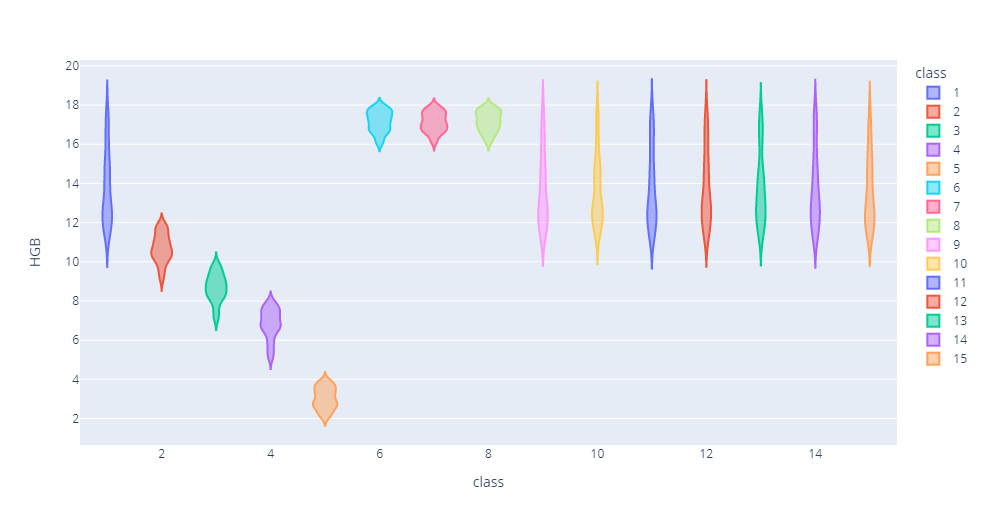
\includegraphics[scale=0.31]{figure4.png}
\label{vplot}
\caption{Violin plot for HGB \& class}
\end{figure}
\pagebreak
\begin{figure}[ht]
\centering
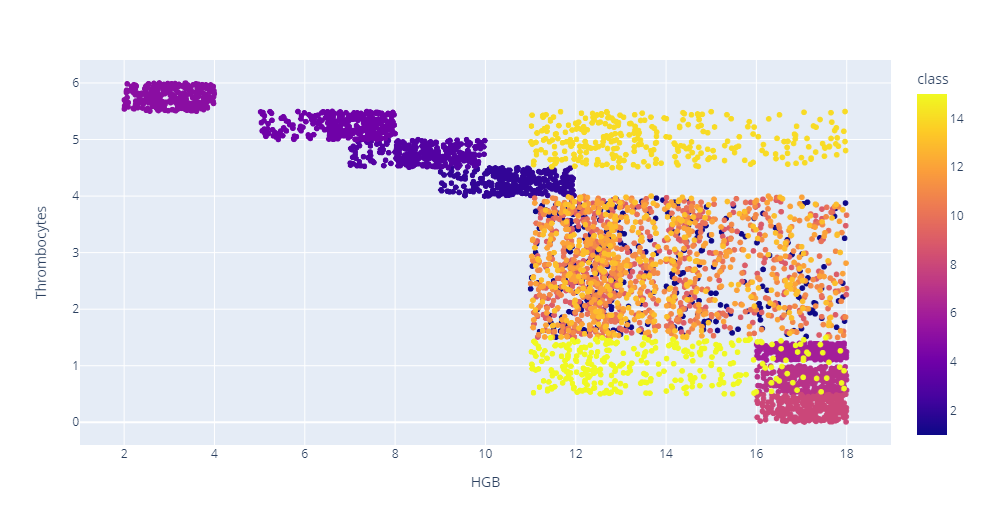
\includegraphics[scale=0.25]{figure5.png}
\label{splot}
\caption{Scatter Plot HGB vs Thrombocytes}
\end{figure}

\begin{center}
\section{WEBSITE}
\end{center}
We also created a web-page to interact with the patient. A start page, in which we can upload an image or a pdf file. OCR recognizes the desired values from the uploaded files and gives those values to the model. The model predicts the disease using those values and displays the disease along with normal parameters, abnormal parameters, symptoms and precautions through a results page.

\vspace{0.5cm}

\begin{figure}[ht]
\centering
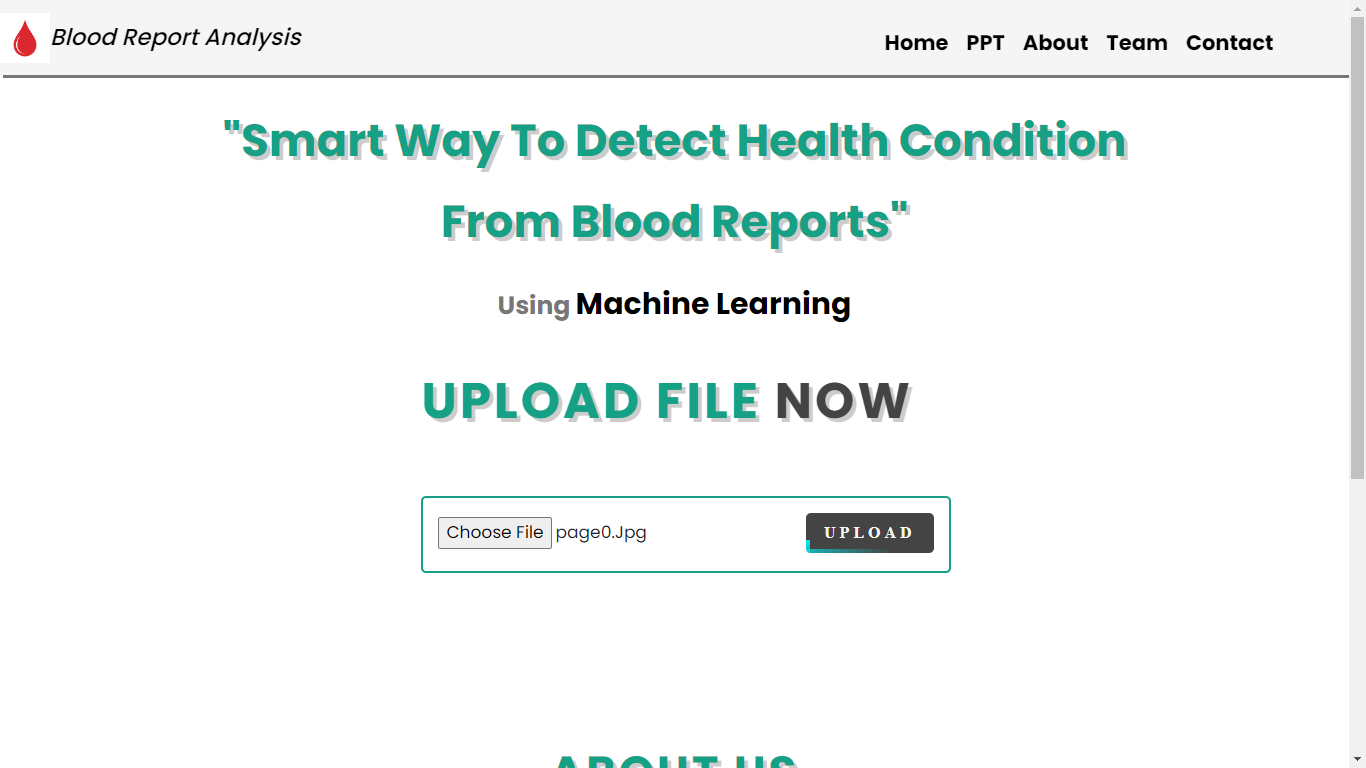
\includegraphics[scale=0.23]{figure6.png}
\label{spage}
\caption{Start Page}
\end{figure}

\vspace{0.7cm}

\begin{figure}[ht]
\centering
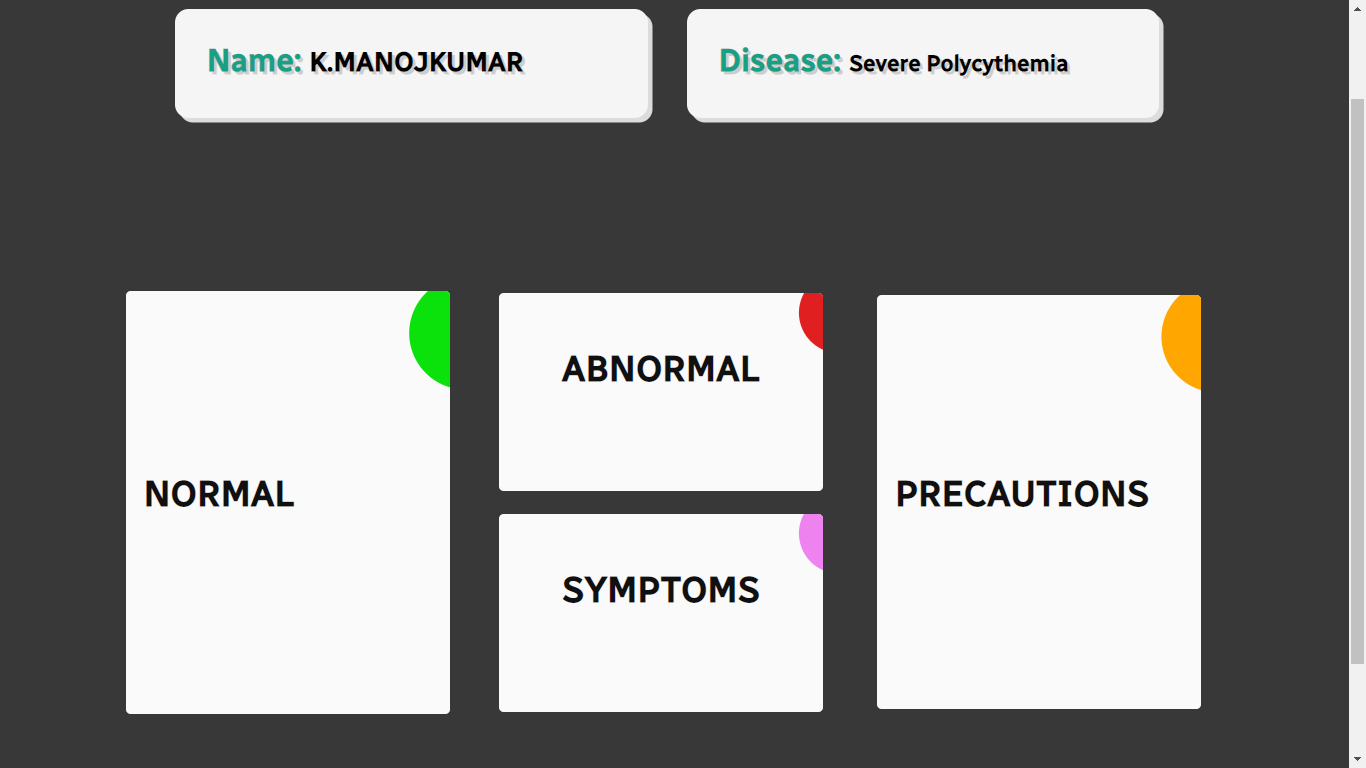
\includegraphics[scale=0.23]{figure7.png}
\label{rpage}
\caption{Results Page}
\end{figure}

\section{ CONCLUSION AND FUTURE WORK}
Machine learning becomes an essential technique for modeling the human process in many disciplines, especially in the medical field, because of the high availability of data. One of the essential disease detectors is the blood analysis; as it contains many parameters with different values that indicate definite proof of the existence of the disease.\cite{Michalski1990}

 The machine learning algorithm accuracy depends mainly on the quality of the dataset; for this reason, a high-quality dataset is collected. This dataset is used for training the classifiers for obtaining high accuracy. We tested several classifiers and achieved accuracy up to 100\% which realizes the research objective, which is helping physicians to predict blood diseases according to a general blood test.\cite{Park2016} 
 
The future work will focus on testing the proposed data set using different deep learning algorithms to compare classical and deep learning approaches in this research area.\cite{Suykens1999}


\bibliographystyle{IEEEtran}
\bibliography{references}

\end{document}